
\begin{center}
\Huge
Potensvækst og potensfunktioner
\end{center}
\section*{Potensfunktioner}
\stepcounter{section}

I har allerede tidligere set et eksempel på en potensfunktion: Et polynomium på formen $f(x) = ax^2$. Mere generelt har vi følgende definition på potensfunktioner:
\begin{defn}
For $b>0$ og $a\in \mathbb{R}$, så kalder vi en funktion $f$ på formen 
\begin{align*}
f(x) = b\cdot x^a
\end{align*}
for en potensfunktion. En variabelsammenhæng $y=b\cdot x^a$ kaldes tilsvarende for en potenssammenhæng.
\end{defn}

\begin{exa}
Et rektangel med bredde $x$ og længde $2\cdot x$ har areal $A(x) = 3\cdot x\cdot x = 3\cdot x^2$, hvilket er en potensfunktion med $b=3$ og $a=2$
\end{exa}
\begin{exa}
En kasse med bredde $x$, længde $2x$ og højde $3x$ har rumfang $R(x) = 3\cdot x \cdot 2\cdot x\cdot x = 6\cdot x^3$, hvilket er en potensfunktion med $b = 6$ og $a=3$.
\end{exa}

\begin{exa}\label{exa:radio}
I Tabel \ref{tab:radio} fremgår antallet af målinger af radioaktivitet per sekund som funktion af afstanden til et radioaktivt emne. Vi forventer, at dette kan beskrives som en potenssammenhæng. 
\begin{table}[H]
\center
\begin{tabular}{c|c|c|c|c|c|c|c|c|c}
d (cm) & 10 & 20 & 30 & 40 & 50 & 60 & 70 & 80 & 90\\ \hline
A & 121 & 80 & 63 & 44 & 44 & 30 & 30 & 23 & 20 
\end{tabular}
\caption{Antal aktiveringer af Geigertæller per sekund som funktion af afstand til radioaktivt emne.}
\label{tab:radio}
\end{table}
Af Fig. \ref{fig:potensreg} kan vi se en potensregression lavet i Maple på radioaktivitetsdatasættet. 
\begin{figure}[H]
\includegraphics[width=\textwidth]{Billeder/potensreg.png}
\caption{Potensregression på radioaktivitetsdata.}
\label{fig:potensreg}
\end{figure}
\end{exa}
Af Fig. \ref{fig:potensfunk} kan de ses, hvad $a$ betyder for en potensfunktion.
\begin{figure}[H]
\centering
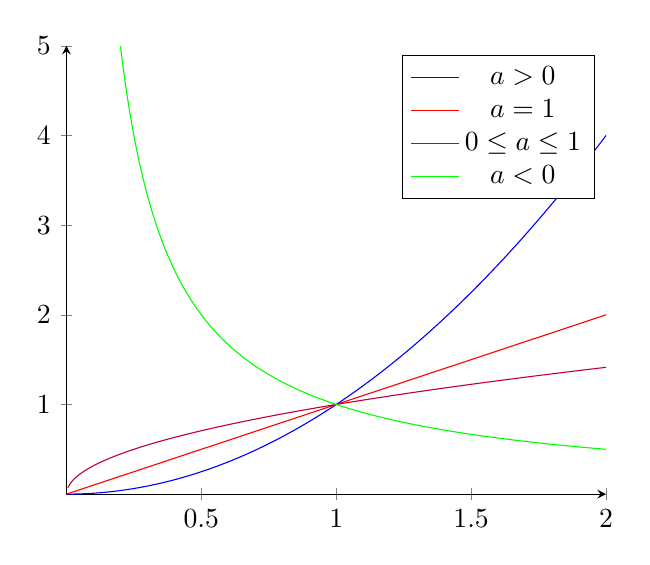
\begin{tikzpicture}
\begin{axis}[axis lines = middle, xmin = 0,xmax = 2]
\addplot[color=blue, samples = 1000] {x^2};
\addlegendentry{$a>0$}
\addplot[color=red,samples = 1000] {x};
\addlegendentry{$a=1$}
\addplot[color=purple,samples = 1000] {sqrt(x)};
\addlegendentry{$0\leq a \leq 1$}
\addplot[color=green, samples = 1000, domain = 0.2:2] {1/x};
\addlegendentry{$a<0$}
\end{axis}
\end{tikzpicture}
\caption{Figur, der viser, hvad $a$ betyder for potensfunktionen}
\end{figure}

Potensfunktioner har mængden $]0,\infty[$ som både definitionsmængde og værdimængde (også kaldet domæne og codomæne). I fald $a = 0$, så er domænet kun $b$. 

\section*{Opgave 1}
\begin{enumerate}[label=\roman*)]
\item Brug regressionen fra Eksempel \ref{exa:radio} til at bestemme antallet af aktiveringer med Geigertælleren der vil være ved 2 meters afstand.
\item Brug regressionen til at bestemme ved hvilken afstand, der er 100 aktiveringer i sekundet. 
\end{enumerate}
\section*{Opgave 2}
Det oplyses, at sammenhæng mellem et penduls længde og svingningstid kan beskrives som en potensfunktion. Data er opsamlet i følgende tabel:

\begin{center}\begin{tabular}{c|c|c|c|c|c}
Længde (m)& 0.5 & 0.75 & 1.00 & 1.25 & 1.50\\ \hline
Svingningstid (s) & 1.4 & 1.7 & 2.1 & 2.2 & 2.5 
\end{tabular}
\end{center}
\begin{enumerate}[label=\roman*)]
\item Lav potensregression på data fra tabellen. 
\item Bestem, hvor lang svingningstiden er, hvis pendulet er 3m
\item Bestem, hvad pendullængden skal være, hvis svingningstiden skal være 4 sekunder. 
\end{enumerate}
\section*{Opgave 3}
\begin{enumerate}[label=\roman*)]
\item En cylinder har samme diameter som højde. Bestem den potensfunktion, der beskriver rumfanget af cylinderen som funktion af cylinderens radius. 
\item En kasse har bredde, højde og længde $x$. Bestem rumfanget af $x$, og afgør, hvad $a$ og $b$ er i denne potensfunktion.
\item For et bestemt objekt kan vindmodstanden på objektet beskrives ved 
\begin{align*}
F(v)= \frac{1}{2}v^2,
\end{align*}
hvor $v$ er hastigheden i $m/s$, objektet bevæger sig med, og $F$ er vindmodstanden målt i $N$. Hvad er vindmodstanden, når objektet bevæger sig med 50$m/s$? Hvor hurtigt skal objektet bevæge sig, for at modstanden på objektet er 20$N$?

\end{enumerate}